\documentclass{beamer}
\usetheme{metropolis}
\usepackage{graphicx}
\usepackage{subfig}
\usepackage{tcolorbox}
\title{Algebra-Based Physics-2: Electricity, Magnetism, and Thermodynamics (PHYS135B): Unit 4}
\author{Jordan Hanson}
\institute{Whittier College Department of Physics and Astronomy}

\begin{document}
\maketitle

\section{Summary}

\begin{frame}{Summary}
\begin{enumerate}
\item Induced emf and magnetic flux
\item Faraday's Law of Induction
\item Motional emf
\item Application: AC generators (PhET)
\end{enumerate}
\end{frame}

\section{Induced emf and magnetic flux}

\begin{frame}{Induced emf and magnetic flux}
\begin{figure}
\centering
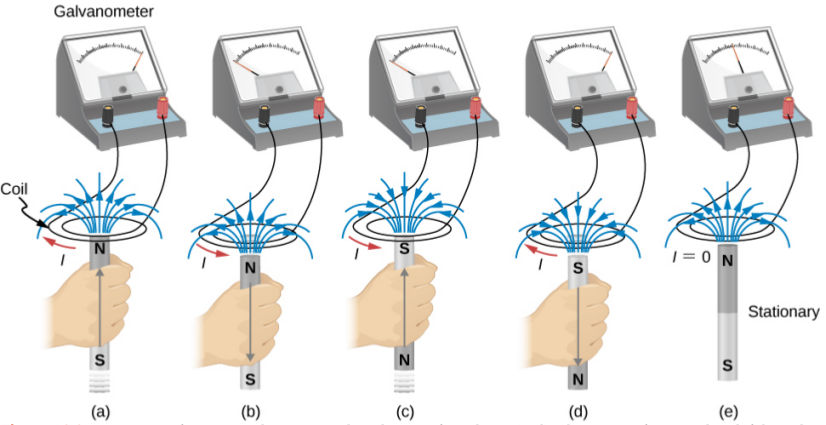
\includegraphics[width=0.9\textwidth]{figures/farad.png}
\caption{\label{fig:farad1} Not only does moving charge create B-fields, but B-fields can create moving charge.  Study each of the cases above, and (Professor) define the concept of \textit{magnetic flux}.}
\end{figure}
\end{frame}

\begin{frame}{Induced emf and magnetic flux}
\begin{figure}
\centering
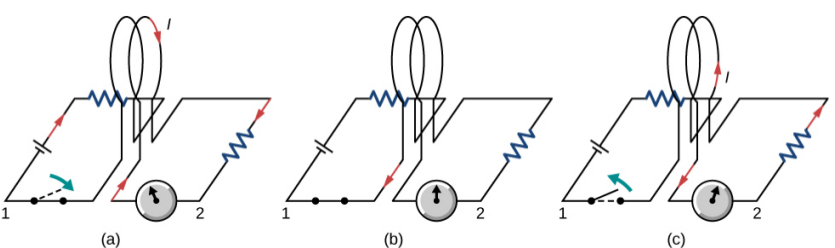
\includegraphics[width=0.9\textwidth]{figures/farad2.png}
\caption{\label{fig:farad2} In addition to a moving magnetic field, \textit{other circuits} can make current flow in a circuit.  The effect must have something to do with \textit{changing} magnetic fields.}
\end{figure}
\end{frame}

\begin{frame}{Induced emf and magnetic flux}
\begin{figure}
\centering
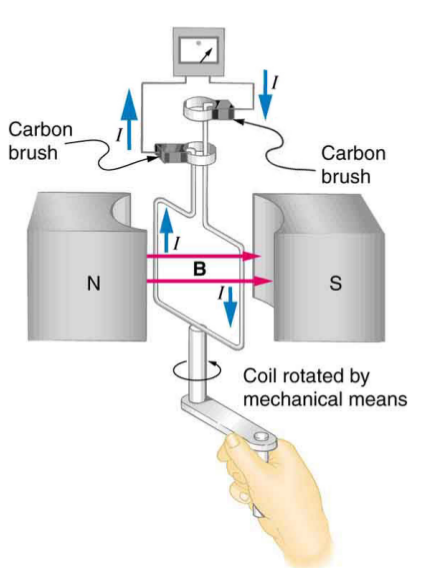
\includegraphics[width=0.3\textwidth]{figures/motorz.png}
\caption{\label{fig:motorz} An AC generator changes mechanical work into electrical energy.}
\end{figure}
\end{frame}

\begin{frame}{Induced emf and magnetic flux}
\begin{figure}
\centering
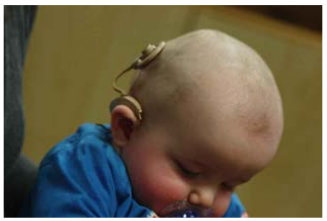
\includegraphics[width=0.6\textwidth]{figures/baby.png}
\caption{\label{fig:baby} A cochlear implant relies on induced emf to power a circuit inside the baby, allowing her to hear.}
\end{figure}
\end{frame}

\begin{frame}{Induced emf and magnetic flux}
Introduction of the concepts:
\url{https://youtu.be/pQp6bmJPU_0}
\end{frame}

\section{Faraday's Law of Induction}

\begin{frame}{Faraday's Law}
\begin{tcolorbox}[colback=white,colframe=black!40!black,title=Faraday's Law]
\alert{The emf $\epsilon$ induced is the negative change in the magnetic flux $\Phi_m$ per unit time. Any change in the magnetic field
or change in orientation of the area of the coil with respect to the magnetic field induces a voltage (emf).
\begin{align}
\phi_m &= \vec{B} \cdot \vec{A} \\
\epsilon &= - \frac{\Delta\phi_m}{\Delta t}
\label{eq:farad}
\end{align}}
\end{tcolorbox}
\textit{The unit of magnetic flux is the Webter, or 1 Wb = 1 T m$^2$.}
\end{frame}

\begin{frame}{Faraday's Law}
\small
\textbf{Example:}
A square coil has sides 0.25 m long and is tightly wound with 200 turns of wire. The resistance of the coil 5.0 Ohms. The coil is placed in a spatially uniform magnetic field that is directed perpendicular to the face of the coil and whose magnitude is decreasing by −0.040 T/s. (a) What is the magnitude of the emf induced in the coil? (b) What is the magnitude of the current circulating through the coil?
\begin{figure}
\centering
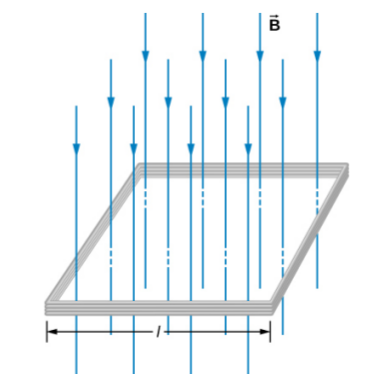
\includegraphics[width=0.3\textwidth]{figures/loop1.png}
\caption{\label{fig:loop1} A 200 turn loop in a B-field.}
\end{figure}
\end{frame}

\begin{frame}{Faraday's Law}
\begin{tcolorbox}[colback=white,colframe=black!40!black,title=Lenz's Law]
\alert{The direction of the induced emf drives current around a wire loop to always oppose the change in magnetic flux that
causes the emf.}
\end{tcolorbox}
\end{frame}

\begin{frame}{Faraday's Law}
\small
\textbf{Example:}
A magnetic field B is directed outward perpendicular to the plane of a circular coil of radius r = 0.50 m.  The field is cylindrically symmetrical with respect to the center of the coil, and its magnitude decreases linearly according to
\begin{equation}
B(t) = B_0 - a t
\end{equation}
with $B_0 = 1.5$ T and $a = 5.0$ T s$^{-1}$.  (a) Calculate the emf induced in the coil at the times $t_0 = 0$, $t_1 = 0.05$, and $t_2 = 1.0$ seconds. (b) Determine the current in the coil if the resistance is 10 Ohms. 
\end{frame}

\begin{frame}{Faraday's Law}
\begin{figure}
\centering
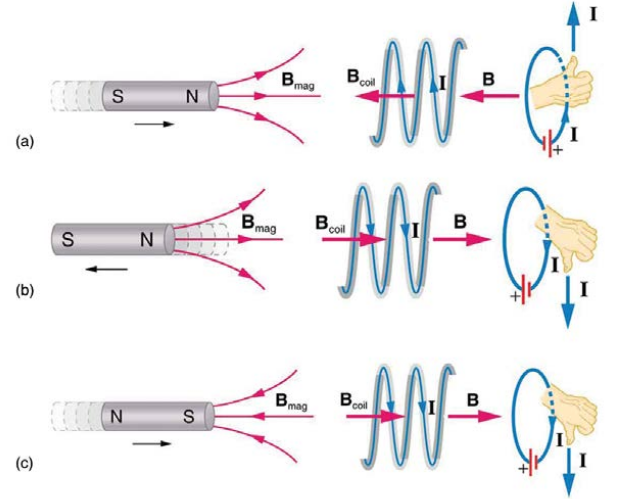
\includegraphics[width=0.6\textwidth]{figures/lenzspecific.png}
\caption{\label{fig:lenz11} A 200 turn loop in a B-field.}
\end{figure}
\end{frame}

\begin{frame}{Faraday's Law}
In the previous example, what would happen if the area $A$ of the loop were increased?
\begin{itemize}
\item A: The current would decrease.
\item B: The current would stay the same.
\item C: The voltage would decrease.
\item D: The voltage would increase.
\end{itemize}
\end{frame}

\begin{frame}{Faraday's Law}
In the previous example, what would happen if the sign $a$ in $B(t)$ were flipped?
\begin{itemize}
\item A: The current would reverse direction and increase in magnitude.
\item B: The current would reverse direction and decrease in magnitude.
\item C: The current would keep the same direction and increase in magnitude.
\item D: The current would keep the same direction and decrease in magnitude.
\end{itemize}
\end{frame}

\begin{frame}{Faraday's Law}
In the previous example, what would happen if $a$ in $B(t)$ were increased?
\begin{itemize}
\item A: The current would reverse direction and increase in magnitude.
\item B: The current would reverse direction and decrease in magnitude.
\item C: The current would keep the same direction and increase in magnitude.
\item D: The current would keep the same direction and decrease in magnitude.
\end{itemize}
\end{frame}

\section{Motional emf}

\begin{frame}{Motional emf}
\small
\begin{figure}
\centering
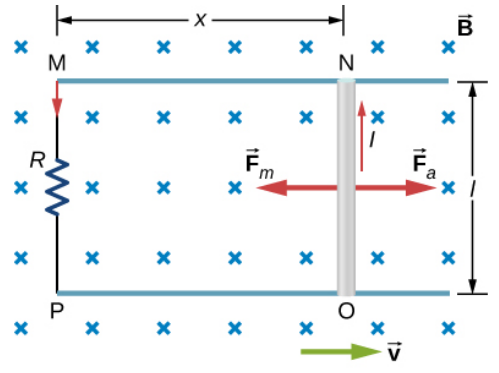
\includegraphics[width=0.5\textwidth]{figures/loop2.png}
\caption{\label{fig:loop4} A system in which the magnetic flux depends on time.}
\end{figure}
\begin{enumerate}
\item Show that power is equal to $P = \vec{F} \cdot \vec{v}$ for constant acceleration.
\item Show that the emf is $\epsilon = B l v$, from Faraday's Law.
\item Show that power generated, $P = I^2 R$, is equal to power injected.
\end{enumerate}
\end{frame}

\begin{frame}{Motional emf}
In the previous example, what would happen if $\vec{F}_a$ was pointed to the left?
\begin{itemize}
\item A: The current would reverse direction.
\item B: The current would keep the same direction.
\item C: The magnetic flux due to the external field would decrease.
\item D: A and C
\end{itemize}
\end{frame}

\begin{frame}{Motional emf}
In the previous example, what would happen if $R$ were increased, but the magnitude and direction of $F_a$ were kept the same?
\begin{itemize}
\item A: The current would decrease.
\item B: The current would increase.
\item C: The current would remain constant.
\item D: The power required would increase.
\end{itemize}
\end{frame}

\begin{frame}{Motional emf}
In the previous example, if mechanical power in the bar is transformed into electrical power (through the resistor), where is the energy stored while it's being transferred?
\begin{itemize}
\item A: The wire.
\item B: No where.
\item C: The B-field.
\item D: The resistor.
\end{itemize}
\end{frame}

\section{Faraday's Law: An application}

\begin{frame}{Faraday's Law: An application}
Start with Faraday's Law:
\begin{equation}
\epsilon = - \frac{\Delta \phi_B}{\Delta t}
\end{equation}
The flux $\phi_B$ is changing and depends on time:
\begin{equation}
\phi_B = \vec{B} \cdot \vec{A}(t) = BA\cos(\theta(t))
\end{equation}
Let the \textit{angular velocity} be constant: $\theta = \omega t$.  Then we have
\begin{equation}
\phi_B  = BA\cos(\omega t)
\end{equation}
Thus the emf (with $N$ loops) is (...calculus...)
\begin{equation}
\epsilon = N\omega BA \sin(\omega t) = \epsilon_0 \sin(\omega t)
\end{equation}
\textbf{The generation of AC power stems from $\omega$.} \\ (Professor: diagram of $\epsilon(t)$).
\end{frame}

\begin{frame}{Faraday's Law: An application}
\begin{equation}
\epsilon = N\omega BA \sin(\omega t)
\end{equation}
The AC voltage equation above is a basic model for the voltage from a generator.  Which of the following would increase the \textit{amplitude} of the emf?
\begin{itemize}
\item A: Turning the area more slowly.
\item B: Turning the area more quickly.
\item C: Increasing the B-field.
\item D: Both B and C.
\end{itemize}
\end{frame}

\begin{frame}{Faraday's Law: An application}
\begin{equation}
\epsilon = N\omega BA \sin(\omega t)
\end{equation}
The AC voltage equation above is a basic model for the voltage from a generator.  Which of the following would increase the \textit{frequency} of the emf?
\begin{itemize}
\item A: Turning the area more slowly.
\item B: Turning the area more quickly.
\item C: Increasing the B-field.
\item D: Both B and C.
\end{itemize}
\end{frame}

\begin{frame}{Faraday's Law: An application}
\begin{equation}
\epsilon = N\omega BA \sin(\omega t)
\end{equation}
\textbf{Group exercise:} Suppose an AC generator rotates at 200 rpm, in a B-field with 0.1 T, and has 100 loops with radius 5 cm.  (a) What is the peak voltage this generator will produce? (b) If the generator powers a system with resistance of 1k$\Omega$, what will be the peak current?
\end{frame}

\section{PhET: AC Power generator}

\begin{frame}{PhET: AC Power generator}
\small
Go to the link: \\ \vspace{0.5cm}
\url{https://phet.colorado.edu/en/simulation/generator}
\end{frame}

\begin{frame}{PhET: AC Power generator}
\small
At left is a water source that falls under gravity, turning a wheel.  Set the water rate with the slider at the top left.  Slide it until the meter reads 10 rotations per minute.
\begin{enumerate}
\item Under the pickup coil menu, choose the voltage meter.
\item Under loops, choose 1 loop, and under area, leave it at 50\%.  Leave the strength of the bar magnet as is.
\item Choose show field meter in the upper right, and place the measurement tool in the center of the loops.
\item Draw a graph of the average B-field versus time.
\item Underneath the graph of B-field versus time, draw a graph of the voltage versus time in the pickup coil.
\item Change the number of loops to 3, and add a new B-field curve to the original B-field vs. time plot, and add a new curve to the original voltage versus time plot.
\end{enumerate}
\end{frame}

\begin{frame}{PhET: AC Power generator}
\small
\textbf{Now double the water rate to 20 rpm, and create a new set of graphs:}
\begin{enumerate}
\item Under loops, choose 1 loop, and under area, leave it at 50\%.  Leave the strength of the bar magnet as is.
\item Draw a graph of the average B-field versus time.
\item Underneath the graph of B-field versus time, draw a graph of the voltage versus time in the pickup coil.
\item Change the number of loops to 3, and add a new B-field curve to the original B-field vs. time plot, and add a new curve to the original voltage versus time plot.
\end{enumerate}
\textbf{Which of your graphs should be the same as the 10 rpm case, and which should be different?}
\end{frame}

\section{Transformers}

\begin{frame}{Transformers}
\small
\begin{figure}
\centering
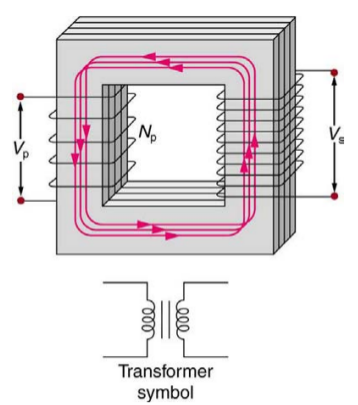
\includegraphics[width=0.4\textwidth]{figures/trans.png}
\caption{\label{fig:trans1} A \textit{transformer} uses Faraday's law to change voltages in AC-generated systems.}
\end{figure}
\begin{equation}
\frac{V_2}{V_1} = \frac{N_2}{N_1}
\end{equation}
\end{frame}

\begin{frame}{Transformers}
\small
\begin{figure}
\centering
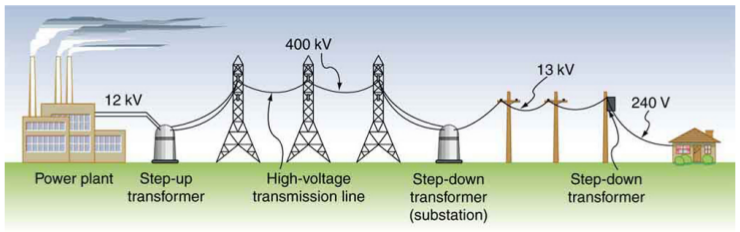
\includegraphics[width=0.9\textwidth]{figures/trans2.png}
\caption{\label{fig:trans2} An example of a distributed power-grid operating on AC principles with step-up and step-down transformers.}
\end{figure}
\end{frame}

\section{Conclusion}

\begin{frame}{Summary}
\textbf{Reading: Chapters 23.1-23.3} \\ \vspace{0.5cm}
\begin{enumerate}
\item 23.1: Induced emf and magnetic flux
\item 23.2: Faraday's Law of Induction
\item 23.3: Motional emf
\item Application: AC generators (PhET)
\end{enumerate}
\end{frame}

\end{document}
